\documentclass[12pt, a4paper]{article}
\title{Algorytmy hashowania}
\author{Student \thanks{III roku Informatyki}}
\date{Kwiecień 2024}
\usepackage{graphicx} %LaTeX package to import graphics
\graphicspath{{}} %configuring the graphicx package
\usepackage[utf8]{inputenc}   
\usepackage[polish]{babel}  
\usepackage[T1]{fontenc}    
\usepackage{lmodern,cmap}    
\begin{document}
\maketitle
\newpage
\section{Bcrypt}
\subsection{Historia powstania}

Bcrypt został opracowany przez Nielsa Progera w 1999 roku i został zaprezentowany na konferencji USENIX, która odbyła się w styczniu 1999 roku w San Antonio w Teksasie. Konferencja USENIX to coroczne spotkanie dla specjalistów z dziedziny systemów operacyjnych, sieci komputerowych i bezpieczeństwa. Właśnie na tej konferencji Proger zaprezentował swoją nową funkcję haszującą.
Historia powstania Bcrypt jest związana z potrzebą bezpiecznego przechowywania haseł w systemach UNIX. W tamtych czasach popularne było przechowywanie haseł w pliku /etc/passwd. Hasła były przechowywane w postaci jawnej lub za pomocą prostych funkcji haszujących, co oznaczało, że były one narażone na ataki hakerskie.
W tym czasie Proger pracował jako administrator systemów w Niemczech i zdawał sobie sprawę z ryzyka, jakie wiązało się z przechowywaniem haseł w pliku /etc/passwd. Postanowił więc opracować nową funkcję haszującą, która była by bezpieczniejsza niż istniejące rozwiązania.
Po wielu miesiącach pracy Proger stworzył Bcrypt, który był oparty na algorytmie Blowfish, który został zaprojektowany przez Bruce'a Schneiera w 1993 roku. Algorytm Blowfish był szyfrem symetrycznym, co oznaczało, że ten sam klucz mógł być używany do szyfrowania i deszyfrowania danych. Jednak Proger wykorzystał algorytm Blowfish w sposób innowacyjny, tworząc funkcję haszującą, która była bezpieczna i wydajna.
Podczas prezentacji na konferencji USENIX, Bcrypt został bardzo dobrze przyjęty przez specjalistów z branży bezpieczeństwa. Od tego czasu Bcrypt stał się popularnym algorytmem haszowania, który jest szeroko stosowany w różnych aplikacjach i systemach, zwłaszcza w systemach opartych na UNIX.

\subsection{Co to jest Bcrypt?}

Bcrypt jest jednym z najbardziej popularnych algorytmów haszowania, który jest szeroko stosowany w celu zabezpieczenia haseł i innych poufnych informacji przed atakami hakerskimi. Jest to algorytm oparty na funkcji haszującej, która konwertuje dowolną ilość danych wejściowych na wartość skrótu o stałej długości.
Jednym z największych atutów Bcrypt jest to, że jest on bardzo bezpieczny i odporny na ataki brute-force. Dzięki zastosowaniu specjalnego algorytmu i tzw. "solenia" hasła, Bcrypt jest w stanie skutecznie chronić przed atakami, które polegają na próbie odgadnięcia hasła poprzez przetestowanie wszystkich możliwych kombinacji.
Sama koncepcja "solenia" polega na dodaniu losowo wygenerowanej wartości, zwanej solą, do samego hasła przed jego zahaszowaniem. To zabezpieczenie zapewnia, że nawet jeśli dwa identyczne hasła zostaną zahaszowane, to wartość skrótu będzie różniła się znacząco, dzięki czemu atakujący nie będzie mógł odgadnąć hasła.
Co więcej, Bcrypt jest łatwy w użyciu i jest dostępny w wielu popularnych językach programowania, co czyni go bardzo uniwersalnym narzędziem do zabezpieczania danych. Niektóre popularne języki, które obsługują bCrypt, to Java, Python, Ruby i PHP.
Warto także zaznaczyć, że Bcrypt jest nie tylko bezpieczny, ale także wydajny. Dzięki temu, że algorytm ten został zoptymalizowany pod kątem szybkości, może on być stosowany w różnych zastosowaniach, w tym do szyfrowania haseł w aplikacjach internetowych i mobilnych.
Podsumowując, Bcrypt to algorytm haszowania, który jest jednym z najlepszych narzędzi do zabezpieczania haseł i innych poufnych informacji. Dzięki jego bezpieczeństwu, wydajności i prostocie użycia, jest to popularny wybór dla wielu programistów i firm, które dbają o bezpieczeństwo swoich danych i użytkowników.

\subsection{Key stretching}
Key stretching jest metodą polegającą na zwiększenia kosztu ataku na klucz lub funkcję skrótu.
Metoda ta zazwyczaj polega na wielokrotnym hashowaniu funkcji. Jest to proste w implementacji i daje bardzo dobre efekty. 
Ogólny algorytm przedstawia poniższy listing:

\begin{verbatim}
function multihash(numrounds, password){
        for (i=0; i<numrounds; ++i)
        password = hashfunction(password);
        return password
        }

\end{verbatim}
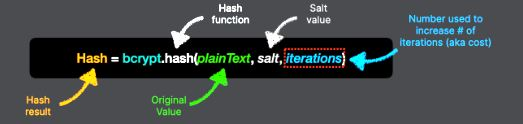
\includegraphics{bcrypt1.JPG}
Metoda ta jest głównie kojarzona z wielokrotnym hashowaniem zwiększającym moc obliczeniową algorytmów. Jest to jednak ogólna technika zwiększająca koszt ataku dowolnej funkcji hashującej czy szyfrującej.
\subsection{Zastosowanie Bcrypt}

Bcrypt może być stosowany w różnych przypadkach, w których potrzebne jest bezpieczne haszowanie haseł i innych poufnych danych. 
Kilka przykładów użycia bCrypt to:
\begin{itemize}
\item \textbf{Systemy autoryzacji i uwierzytelniania:} Bcrypt jest często wykorzystywany do zabezpieczania systemów autoryzacji i uwierzytelniania w aplikacjach internetowych i mobilnych. Dzięki temu użytkownicy mogą bezpiecznie logować się do swoich kont i chronić swoje poufne dane.
\item \textbf{Przetwarzanie transakcji finansowych:} w przypadku aplikacji, które przetwarzają transakcje finansowe, bezpieczeństwo jest kluczowe. Bcrypt może być wykorzystany do haszowania numerów kart kredytowych, numerów kont bankowych i innych poufnych informacji, aby zapewnić, że te dane nie zostaną skradzione lub wykorzystane przez osoby niepowołane.
\item \textbf{Systemy zarządzania hasłami:} Bcrypt może być stosowany do haszowania i przechowywania haseł w systemach zarządzania hasłami, takich jak LastPass czy KeePass. Dzięki temu użytkownicy mogą przechowywać swoje hasła bezpiecznie, bez obawy o to, że zostaną one skradzione lub wykorzystane przez osoby niepowołane.
\item \textbf{Aplikacje korporacyjne:} Bcrypt może być stosowany do zabezpieczania danych w aplikacjach korporacyjnych, takich jak systemy CRM, ERP czy HR. Dzięki temu poufne dane, takie jak dane personalne pracowników, są bezpiecznie przechowywane i chronione przed dostępem osób niepowołanych.
\item \textbf{Serwery gier:} Bcrypt może być wykorzystany do zabezpieczania serwerów gier online, które wymagają autoryzacji graczy. Dzięki temu gracze mogą bezpiecznie logować się i grać, a ich poufne dane, takie jak adresy e-mail i hasła, są chronione przed dostępem osób niepowołanych.
\end{itemize}
To tylko kilka przykładów użycia Bcrypt. Algorytm ten może być stosowany w wielu innych przypadkach, w których potrzebne jest bezpieczne haszowanie danych.
\subsection{Łamanie hasła Bcrypt}
\begin{center}
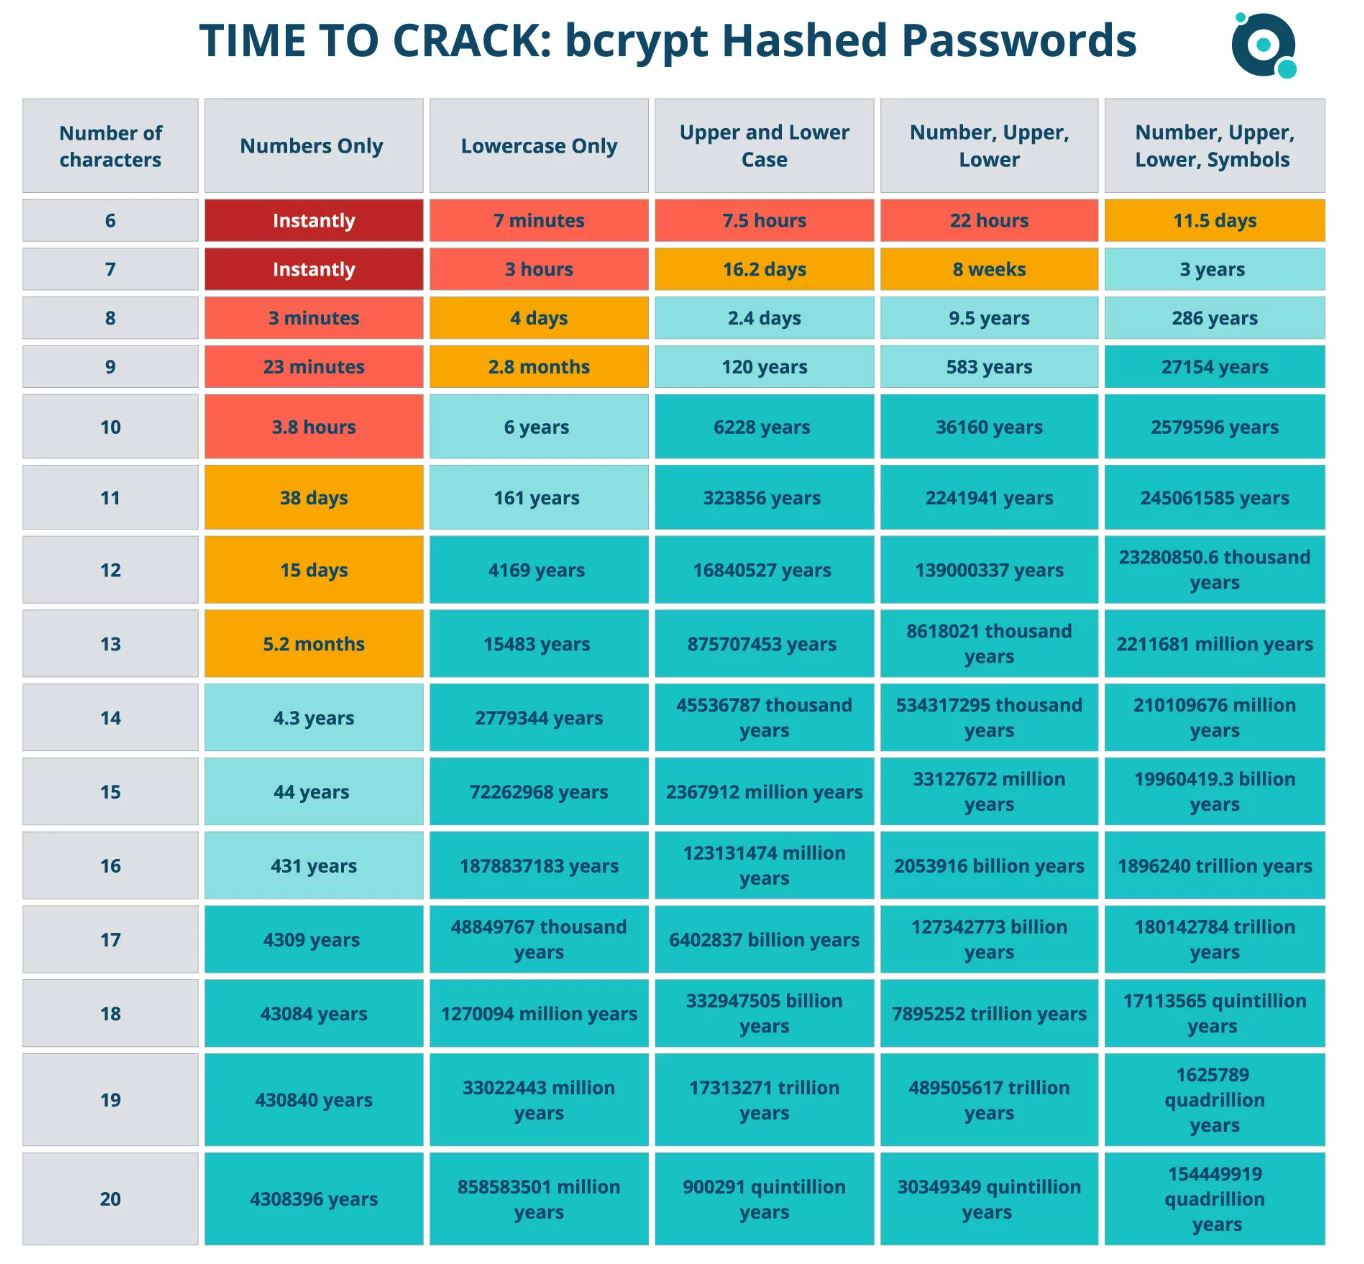
\includegraphics[scale=0.25]{bcrypt2.JPG}
\end{center}
\section{MD5 (Message Digest Algorithm 5)}
\subsection{Historia powstania}
MD5 jest jednym z serii algorytmów zaprojektowanych przez profesora Rona Rivesta z MIT (Rivest, 1994). Poprzednikiem był algorytm MD4, który w wyniku analizy przeprowadzonej przez Hansa Dobbertina okazał się zbyt mało bezpieczny. Jego bezpiecznym następcą był MD5 opracowany w 1991.
W 1996 Dobbertin zaprezentował analizę kolizji algorytmu MD5. Chociaż nie był to jeszcze pełny atak na funkcję skrótu, to jednak wystarczył, aby specjaliści w dziedzinie kryptografii zaczęli stosować silniejsze odpowiedniki, takie jak SHA-1 lub RIPEMD-160.
W marcu 2004 powstał rozproszony projekt nazywany MD5CRK . Twórcą projektu był Jean-Luc Cooke i jego współpracownicy. Miał on na celu wykazanie, że możliwe jest wyznaczenie wiadomości różnej od zadanej, która ma taką samą wartość skrótu. Do tego celu wykorzystano sieć Internet oraz dużą liczbę komputerów biorących udział w projekcie. Projekt wykazał, że dysponując bardzo dużą mocą obliczeniową możliwe jest podrabianie generowanych podpisów.
Dopiero prace badawcze chińskich naukowców Xiaoyun Wang, Dengguo Fen, Xuejia Lai i Hongbo Yu w pełni wykazały słabość algorytmu. 17 sierpnia 2004 opublikowali oni analityczny algorytm ataku, dzięki któremu do podrobienia podpisu wystarczyła godzina działania klastrowego komputera IBM P690.
W marcu 2005 Arjen Lenstra, Xiaoyun Wang i Benne de Weger zaprezentowali metodę umożliwiającą znalezienie kolizji dla algorytmu MD5 i przeprowadzenie ataku polegającego na wysłaniu dwóch różnych wiadomości chronionych tym samym podpisem cyfrowym. Kilka dni później Vlastimil Klima opublikował algorytm, który potrafił znaleźć kolizję w ciągu minuty, używając metody nazwanej tunneling.
Pod koniec 2008 roku niezależni kalifornijscy specjaliści ds. bezpieczeństwa, we współpracy z ekspertami z Centrum voor Wiskunde en Informatica, Technische Universiteit Eindhoven oraz Ecole Polytechnique Fédérale de Lausanne odkryli lukę w MD5 umożliwiającą podrobienie dowolnego certyfikatu SSL w taki sposób, że zostanie on zaakceptowany przez wszystkie popularne przeglądarki internetowe. Do podrobienia certyfikatu wystarczyła moc obliczeniowa 200 konsol do gier PlayStation 3.
Od lat 90. MD5 nie jest uważany za bezpieczny do większości zastosowań i w jego miejsce zaleca się stosowanie algorytmów z rodziny SHA-2 lub SHA-3.
\subsection{Co to jest MD5}
MD5 (z ang. Message-Digest algorithm 5) – algorytm kryptograficzny, opracowany przez Rona Rivesta (współtwórcę RSA) w 1991 roku, będący popularną kryptograficzną funkcją skrótu, która z ciągu danych o dowolnej długości generuje 128-bitowy skrót.
W 2004 znaleziono sposób na generowanie kolizji MD5, co obniża jego bezpieczeństwo w niektórych zastosowaniach (np. podpisywaniu plików).
Z powodu znanych ataków kryptoanalitycznych funkcja MD5 zdecydowanie nie powinna być używana w zastosowaniach wymagających odporności na kolizje, na przykład w podpisie cyfrowym. W innych, takich jak HMAC, nadal może zapewniać satysfakcjonujący poziom bezpieczeństwa, choć stosowanie jej w nowych rozwiązaniach nie jest zalecane.
\subsection{Algorytm MD5}
Algorytm MD5 jest następujący:
\begin{itemize}
\item Doklejenie do wiadomości wejściowej bitu o wartości 1
\item Doklejenie takiej ilości zer, by ciąg składał się z 512-bitowych bloków i ostatniego niepełnego – 448-bitowego
\item Doklejenie 64-bitowego (zaczynając od najmniej znaczącego bitu) licznika oznaczającego rozmiar wiadomości; w ten sposób otrzymywana wiadomość złożona jest z 512-bitowych fragmentów
\item Ustawienie stanu początkowego na 0123456789abcdeffedcba9876543210
\item Uruchomienie na każdym bloku funkcji zmieniającej stan (istnieje przynajmniej jeden blok nawet dla pustego wejścia)
\item Zwrócenie stanu po przetworzeniu ostatniego bloku jako obliczony skrót wiadomości
\end{itemize}
Funkcja zmiany stanu ma 4 cykle (64 kroki). Stan jest traktowany jako 4 liczby 32-bitowe. W każdym kroku do jednej z tych liczb dodawany jest jeden z 16 32-bitowych fragmentów bloku wejściowego, pewna stała zależna od numeru kroku oraz pewna prosta funkcja boolowska 3 pozostałych liczb. Następnie liczba ta jest obracana (przesuwana cyklicznie z najstarszymi bitami wsuwanymi w najmłodsze pozycje) o liczbę bitów zależną od kroku oraz jest dodawana do niej jedna z pozostałych liczb.
\subsection{Do czego służy MD5}
Mimo znanych problemów związanych z bezpieczeństwem, MD5 nadal jest używany do hashowania haseł w oprogramowaniu. MD5 służy do przechowywania haseł za pomocą jednokierunkowego hasha hasła, ale nie należy do zalecanych funkcji haszujących do tego celu. MD5 jest powszechnie stosowany i łatwy w użyciu, dlatego programiści często wciąż wybierają go do hashowania i przechowywania haseł.
MD5 jest również nadal wykorzystywany w cyberbezpieczeństwie do weryfikacji i uwierzytelniania cyfrowych podpisów. Korzystając z MD5, użytkownik może zweryfikować, czy pobrany plik jest autentyczny, dopasowując klucz publiczny i prywatny oraz wartości skrótu. Ze względu na wysoką liczbę kolizji w MD5, jednakże, ten algorytm funkcji skrótu nie jest idealny do weryfikowania integralności danych lub plików, ponieważ atakujący mogą łatwo zastąpić wartość skrótu własną.
Dane mogą być weryfikowane pod kątem integralności za pomocą MD5 jako funkcji sumy kontrolnej, aby upewnić się, że nie zostały przypadkowo uszkodzone. Pliki mogą wykazywać błędy, gdy zostaną niezamierzenie zmienione w jednym z następujących sposobów:
\begin{itemize}
\item Błędy w transmisji danych
\item Błędy oprogramowania
\item Podczas kopiowania lub przenoszenia plików mogą wystąpić błędy zapisu
\item Problemy z nośnikiem danych
\end{itemize}
Algorytm wiadomości skrótu MD5 może być używany do zapewnienia, że dane są takie same, jakie były pierwotnie, sprawdzając, czy wynik jest taki sam jak dane wejściowe. Jeśli plik został niezamierzony zmieniony, dane wejściowe utworzą inny skrót, który już nie będzie pasował. Oznacza to, że plik jest uszkodzony. Jest to skuteczne tylko wtedy, gdy dane zostały niezamierzony uszkodzone, jednakże nie w przypadku celowego manipulowania nimi.
\subsection{Łamanie hasła MD5}
\begin{center}
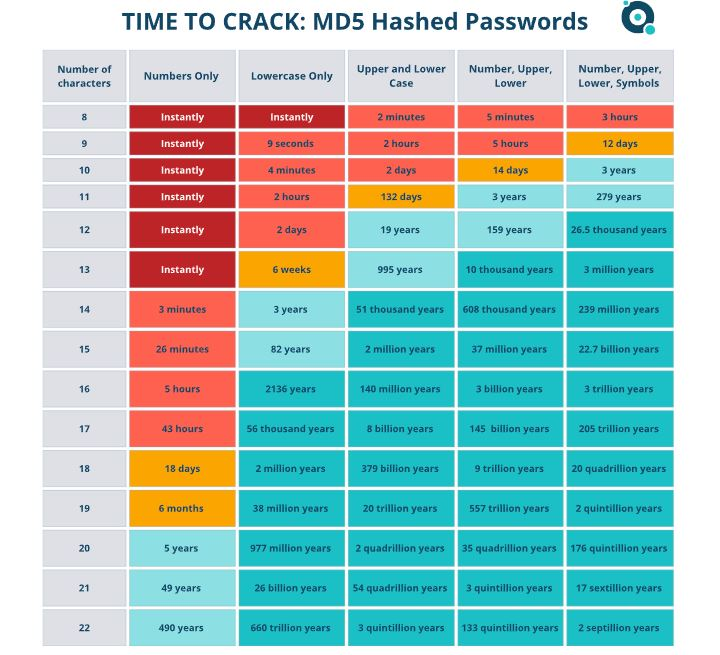
\includegraphics[scale=0.50]{md5.JPG}
\end{center}
\section{SHA-256 (Secure Hash Algorithm 256-bit)}
\subsection{Historia powstania}
Secure Hash Algorithm 256-bit (SHA-256) to powszechnie stosowana funkcja skrótu kryptograficznego, która generuje stały wynik o długości 256 bitów dla różnych danych wejściowych. Należy ona do rodziny funkcji skrótu SHA-2, której poprzedziły najwcześniejsze funkcje skrótu SHA-1. Wyższe liczby oznaczają długość wyników skrótu, o czym będziemy rozmawiać poniżej.
Początki SHA-256 można śledzić do służb wywiadowczych w USA, a mianowicie do Narodowej Agencji Bezpieczeństwa, czyli NSA. Inżynierowie zatrudnieni w agencji dużo inwestowali w rozwój algorytmu i po raz pierwszy opublikowali go w 2001 roku. Głównym celem stworzenia SHA-256 było zoptymalizowanie wcześniejszych funkcji skrótu, takich jak MD5 i SHA-1, które okazały się podatne na kilka znanych wektorów ataku.
Co ciekawe, SHA-256 jest szeroko stosowany w cyberbezpieczeństwie, w tym w cyfrowych podpisach, przechowywaniu haseł i kodach uwierzytelniania wiadomości. Został także wykorzystany w algorytmach konsensusu proof-of-work używanych w blockchainach, takich jak Bitcoin, na przykład.
Algorytm operuje na danych wejściowych w fragmentach, zwanych blokami, i przetwarza je poprzez serię operacji matematycznych. Wynikiem SHA-256 jest skrót 256-bitowy, stąd nazwa, który jest unikalny dla każdego unikalnego wejścia.
Jedną z głównych cech SHA-256 jest jego odporność na ataki kolizyjne, co oznacza, że jest obliczeniowo niemożliwe wygenerowanie tego samego wyniku hashowania z dwóch różnych danych wejściowych. Innymi słowy, wyniki mogą być sprawdzane retrospektywnie, ponieważ ich wyniki zawsze będą odpowiadać unikalnemu zestawowi danych wejściowych.
Jednakże jest także odporne na preobrazowanie, co czyni praktycznie niemożliwym wywnioskowanie prywatnych kluczy nadawcy z wartości skrótu transakcji. Dlatego zarówno klucze publiczne, jak i prywatne są używane równocześnie dla synergii przejrzystości i bezpieczeństwa.
\subsection{Do czego jest używany SHA-256}
\begin{itemize}
\item \textbf{Weryfikacja cyfrowych podpisów:} Cyfrowe podpisy stosują metodologię szyfrowania asymetrycznego w celu weryfikacji autentyczności dokumentu/pliku. Algorytmy skrótu, takie jak SHA-256, odgrywają ważną rolę w zapewnieniu weryfikacji podpisu.
\item \textbf{Haszowanie haseł:} Strony internetowe przechowują hasła użytkowników w postaci zahaszowanej z dwóch powodów. Pomaga to budować poczucie prywatności i zmniejsza obciążenie na centralnej bazie danych, ponieważ wszystkie skróty są podobnego rozmiaru.
\item \textbf{Handshake SSL:} Handshake SSL to kluczowy segment sesji przeglądania stron internetowych, który jest wykonywany za pomocą funkcji SHA. Składa się on z uzgadniania kluczy szyfrowania i autentykacji skrótu między twoją przeglądarką internetową a serwerami internetowymi w celu przygotowania bezpiecznego połączenia.
\item \textbf{Sprawdzanie integralności:} Weryfikacja integralności plików korzysta z wariantów algorytmu SHA-256 i algorytmu MD5. Pomaga to zachować pełną funkcjonalność plików i zapewnić, że nie zostały one zmienione w trakcie transmisji.
\end{itemize}
\section{SHA-3 (Secure Hash Algorithm 3)}
\subsection{Historia powstania}
Historia powstania SHA-3 sięga początków XXI wieku, kiedy to zidentyfikowano podatności w istniejących funkcjach skrótu, takich jak SHA-1 i SHA-2. W 2007 roku Narodowy Instytut Standaryzacji i Technologii (NIST) w Stanach Zjednoczonych ogłosił publiczny konkurs na opracowanie nowej funkcji skrótu kryptograficznego, która mogłaby zastąpić dotychczasowe algorytmy.
Konkurs ten przyciągnął uwagę kryptografów z całego świata, którzy zgłosili liczne propozycje. Po wielu latach analizy i testowania różnych kandydatów, w 2012 roku algorytm Keccak został wybrany jako zwycięzca konkursu. Algorytm ten został zaprojektowany przez belgijskich kryptografów - Guido Bertoni, Joan Daemen, Michaël Peeters i Gilles Van Assche.
Po wyborze algorytmu Keccak nastąpił proces standaryzacji i opracowania szczegółów dotyczących funkcji SHA-3. Ostatecznie, w 2015 roku NIST ustandaryzował Keccak jako SHA-3, co oznaczało jego oficjalne wdrożenie jako nowej funkcji skrótu kryptograficznego.
SHA-3 jest uważane za istotny krok naprzód w dziedzinie kryptografii, ponieważ zapewnia nową warstwę bezpieczeństwa w porównaniu do starszych funkcji skrótu, które mogłyby być podatne na ataki związane z postępem technologicznym i rosnącą mocą obliczeniową.
\subsection{Zastosowanie SHA-3}
\begin{itemize}
\item \textbf{Integralność danych:} Poprzez porównanie wartości skrótu przed i po transmisji lub przechowywaniu można wykryć przypadkowe uszkodzenia danych.
\item \textbf{Przechowywanie haseł:} Zamiast przechowywać faktyczne hasła, systemy często przechowują ich wartości skrótu. Podczas logowania system haszuje Twoje dane wejściowe i sprawdza je względem przechowywanego skrótu.
\item \textbf{Cyfrowe podpisy:} Funkcje skrótu są kluczowe w tworzeniu i weryfikowaniu cyfrowych podpisów, które potwierdzają autentyczność i integralność wiadomości lub dokumentu.
\item \textbf{Protokoły kryptograficzne:} Wiele protokołów kryptograficznych, takich jak mechanizmy wymiany kluczy lub generowanie certyfikatów, wykorzystuje funkcje skrótu do swoich operacji.
\end{itemize}
\subsection{Łamanie hasła SHA-256}
Załóżmy algorytm siłowego ataku, który iteruje przez wszystkie możliwe linie o długości 256 bitów (to nie gwarantuje sukcesu, ale zazwyczaj będzie to wystarczające). Musimy więc przetworzyć 
\begin{verbatim}
2^256 wariantów łańcuchów o długości 256 bitów, 
\end{verbatim}
co daje w przybliżeniu
\begin{verbatim}
    3,2 * 10^79 bitów.
\end{verbatim}
    Załóżmy, że mamy pełny dostęp do najlepszego komputera (według listy TOP500 - czerwiec 2019) - IBM Summit. Posiada on około 2,5 miliona procesorów IBM POWER9, a każda taka jednostka może haszować 3,7 Gb danych na sekundę (zgodnie z podręcznikiem użytkownika), co oznacza, że cały klaster w najlepszym przypadku może przetwarzać około 
\begin{verbatim} 
3,7 * 10^9 * 2,5 * 10^6 = 9,25 * 10^15 bitów danych na sekundę.
\end{verbatim}
Zatem potrzebujemy co najmniej 
\begin{verbatim}
3,5 * 10^63 sekund = 1,1 * 10^57 lat. 
\end{verbatim}
Co jest znacznie więcej niż istnieje Ziemia. 
\section{BLAKE2}
\subsection{Historia Powstania}
BLAKE2 to funkcja skrótu kryptograficznego oparta na BLAKE, stworzona przez Jean-Philippa Aumassona, Samuela Nevesa, Zooko Wilcox-O'Hearna i Christiana Winnerleina. Celem projektu było zastąpienie powszechnie używanych, lecz złamanych, algorytmów MD5 i SHA-1 w aplikacjach wymagających wysokiej wydajności w oprogramowaniu. BLAKE2 został ogłoszony 21 grudnia 2012 roku. Dostępna jest implementacja referencyjna na licencji CC0, licencji OpenSSL i licencji Apache 2.0.

\subsection{BLAKE2}
BLAKE2b jest szybszy niż MD5, SHA-1, SHA-2 i SHA-3, na architekturach 64-bitowych x86-64 i ARM. BLAKE2 zapewnia lepsze bezpieczeństwo niż SHA-2 i podobne do SHA-3: odporność na wydłużanie długości, odróżnialność od losowego wyroczni, itp.
BLAKE2 usuwa dodawanie stałych do słów wiadomości z funkcji rundy BLAKE, zmienia dwa stałe obrotu, upraszcza dopełnienie, dodaje blok parametrów, który jest XORowany z wektorami inicjalizacyjnymi, i zmniejsza liczbę rund z 16 do 12 dla BLAKE2b (następca BLAKE-512), oraz z 14 do 10 dla BLAKE2s (następca BLAKE-256).
BLAKE2 obsługuje klucze, sól, personalizację i tryby drzewa skrótu, oraz może generować skróty o długości od 1 do 64 bajtów dla BLAKE2b, lub do 32 bajtów dla BLAKE2s. Istnieją również wersje równoległe zaprojektowane dla zwiększenia wydajności na procesorach wielordzeniowych: BLAKE2bp (4-sposobowa równoległość) i BLAKE2sp (8-sposobowa równoległość).
BLAKE2X to rodzina funkcji wyjściowych rozszerzalnych (XOFs). Podczas gdy BLAKE2 jest ograniczony do skrótów 64-bajtowych, BLAKE2X pozwala na skróty o wielkości do 256 GiB. BLAKE2X nie jest samodzielną funkcją skrótu, i musi być oparta na rzeczywistej instancji BLAKE2. Przykładem instancji BLAKE2X może być BLAKE2Xb16MiB, który byłby wersją BLAKE2X opartą na BLAKE2b, produkującą skróty 16 777 216 bajtów (dokładnie 16 MiB, stąd nazwa takiej instancji).
BLAKE2b i BLAKE2s są określone w RFC 7693. Opcjonalne funkcje wykorzystujące blok parametrów (solenie, spersonalizowane skróty, skróty drzewa itp.) nie są określone, i dlatego nie ma wsparcia dla BLAKE2bp, BLAKE2sp lub BLAKE2X.
\subsection{Zastosowanie BLAKE2}
BLAKE2 jest stosowany w szerokim zakresie zastosowań w kryptografii i bezpieczeństwie informatycznym, głównie jako funkcja skrótu kryptograficznego. Oto kilka przykładów jego zastosowań:
\begin{itemize}
\item \textbf{Haszowanie haseł:} BLAKE2 często jest wykorzystywany do bezpiecznego haszowania haseł użytkowników przed ich przechowywaniem w systemach informatycznych. Zapewnia to ochronę przed atakami typu "odwrócenie hasła", gdyby dane zostały skradzione.

\item \textbf{Integralność danych:} Jest wykorzystywany do sprawdzania integralności danych poprzez generowanie skrótów dla plików lub danych i porównywanie ich z wcześniejszymi skrótami. Jeśli skróty się różnią, oznacza to, że dane zostały zmienione lub uszkodzone.

\item \textbf{Cyfrowe podpisy:} BLAKE2 może być używany w procesie tworzenia i weryfikacji cyfrowych podpisów, co pomaga w potwierdzeniu autentyczności i integralności wiadomości lub dokumentów.

\item \textbf{Protokoły kryptograficzne:} Funkcja ta może być wykorzystywana w różnych protokołach kryptograficznych, takich jak protokoły wymiany kluczy czy generowania certyfikatów.

\item \textbf{Bezpieczne haszowanie plików:} BLAKE2 może być również stosowany do bezpiecznego haszowania plików, co umożliwia szybkie porównywanie dużych zbiorów danych bez konieczności przechowywania oryginalnych plików.

\item \textbf{Aplikacje blockchain:} W niektórych systemach blockchain BLAKE2 jest wykorzystywany do generowania skrótów bloków, transakcji lub innych danych, co pomaga w weryfikacji ich integralności i autentyczności.
\end{itemize}
Ogólnie rzecz biorąc, BLAKE2 jest używany wszędzie tam, gdzie wymagane jest szybkie, bezpieczne i efektywne haszowanie danych w celu zapewnienia ich integralności, autentyczności i poufności.
\subsection{Łamanie hasła BLAKE2}
Blake2 jest bezpieczną funkcją kryptograficzną, zaprojektowaną tak, aby oprzeć się takim atakom.
\begin{itemize}
\item \textbf{Funkcja jednokierunkowa:} Blake2 tworzy unikalny skrót dla danego wejścia danych, ale odwrócenie tego procesu w celu uzyskania oryginalnych danych jest obliczeniowo niemożliwe.
\item \textbf{Kolizje:} Znalezienie dwóch różnych danych wejściowych, które generują ten sam skrót Blake2, jest niezwykle trudne. Zapobiega to atakującym podstawianiu sfałszowanej wiadomości z tym samym skrótem co legalna wiadomość.
\end{itemize}
Czas potrzebny na złamanie Blake2 metodą brute force byłby astronomiczny. Wiązałoby się to z wypróbowaniem wszystkich możliwych kombinacji znaków, aż do znalezienia takiej, która generuje pożądany skrót. Jest to niepraktyczne przy obecnej technologii.
\section{Wnioski}
Algorytmy haszujące są niezwykle istotne w dzisiejszych systemach informatycznych, zarówno pod względem bezpieczeństwa danych, jak i efektywności przetwarzania. Wybór odpowiedniego algorytmu haszującego zależy od konkretnego zastosowania i wymaga dokładnej analizy wymagań systemu. Ponadto, należy stale monitorować postęp w dziedzinie kryptografii, aby zapewnić, że wykorzystywane algorytmy są nadal bezpieczne i efektywne.
\section{Odniesienia}

\begin{itemize}
\item https://davidburdelak.pl/blog/bcrypt-bezpieczne-przechowywanie-hasla-w-bazie-danych
\item https://bcrypt.online/
\item https://en.wikipedia.org/wiki/Bcrypt
\item https://sekurak.pl/kompendium-bezpieczenstwa-hasel-atak-i-obrona-czesc-3/
\item https://cybr.com/certifications-archives/key-stretching-concepts-and-algorithms/
\item https://pl.wikipedia.org/wiki/MD5
\item https://www.okta.com/identity-101/md5/
\item https://supra.com/academy/the-nsa-and-bitcoin-origins-of-the-sha-256-hashing-algorithm/
\item https://www.simplilearn.com/tutorials/cyber-security-tutorial/sha-256-algorithm
\item https://tecadmin.net/what-is-sha3/
\item https://www.blake2.net/
\item https://specopssoft.com/blog/hashing-algorithm-cracking-bcrypt-passwords/
\end{itemize}


\end{document}

% odnosniki
